\documentclass[aspectratio=169,11pt]{beamer}

% -------------------------------------------------------------
% Academic Presentation Styling (Clean, Minimal, Professional)
% -------------------------------------------------------------
\usetheme{Boadilla}
\usecolortheme{default}

% Disable distracting navigation symbols
\setbeamertemplate{navigation symbols}{}

% Flat, unshadowed academic blocks
\setbeamertemplate{blocks}[rounded=false, shadow=false]
\setbeamertemplate{items}[circle]

% Professional Monochrome Academic Palette (Clean Grayscale & Charcoal)
\definecolor{primaryNavy}{RGB}{24, 24, 27}
\definecolor{secondaryNavy}{RGB}{63, 63, 70}
\definecolor{darkCharcoal}{RGB}{24, 24, 27}
\definecolor{mutedGray}{RGB}{248, 250, 252}
\definecolor{ruleGray}{RGB}{226, 232, 240}
\definecolor{alertDarkRed}{RGB}{63, 63, 70}
\definecolor{accentTeal}{RGB}{39, 39, 42}

% Beamer Element Colors
\setbeamercolor{structure}{fg=primaryNavy}
\setbeamercolor{frametitle}{fg=primaryNavy, bg=white}
\setbeamercolor{title}{fg=primaryNavy}
\setbeamercolor{subtitle}{fg=secondaryNavy}
\setbeamercolor{author}{fg=darkCharcoal}
\setbeamercolor{institute}{fg=darkCharcoal!80}
\setbeamercolor{date}{fg=darkCharcoal!80}

% Footline & Infolines (Subtle, uncluttered)
\setbeamercolor{author in head/foot}{fg=white, bg=primaryNavy}
\setbeamercolor{title in head/foot}{fg=white, bg=secondaryNavy}
\setbeamercolor{date in head/foot}{fg=white, bg=primaryNavy}

% Academic Block Styling
\setbeamercolor{block title}{fg=white, bg=primaryNavy}
\setbeamercolor{block body}{fg=darkCharcoal, bg=mutedGray}
\setbeamercolor{block title alerted}{fg=white, bg=alertDarkRed}
\setbeamercolor{block body alerted}{fg=darkCharcoal, bg=alertDarkRed!8}
\setbeamercolor{block title example}{fg=white, bg=secondaryNavy}
\setbeamercolor{block body example}{fg=darkCharcoal, bg=secondaryNavy!8}

% Frame Title Customization: Clean Title + Thin Divider Rule
\setbeamertemplate{frametitle}{%
    \vspace{0.25cm}%
    \usebeamerfont{frametitle}\insertframetitle%
    \par\vspace{0.15cm}%
    {\color{ruleGray}\hrule height 0.6pt}%
    \vspace{0.1cm}%
}

% Essential Packages
\usepackage[utf8]{inputenc}
\usepackage{amsmath,amssymb}
\usepackage{graphicx}
\usepackage{booktabs}
\usepackage{hyperref}
\usepackage{tikz}
\usetikzlibrary{shapes.geometric, arrows.meta, positioning, calc, fit, backgrounds}

% Graphics Path
\graphicspath{{figures/}{../figures/}}

% Clean Hyperlinks
\hypersetup{
    colorlinks=true,
    linkcolor=primaryNavy,
    urlcolor=primaryNavy,
    citecolor=primaryNavy
}

% Presentation Metadata
\title[Face Reenactment (FOMM)]{Exploring DeepFakes: Face Reenactment}
\subtitle{Comparative Architecture Analysis, FOMM \& Failure Mode Experiments}
\author[Arslan et al.]{Yusuf Arslan \and Erdem Çelikel \and [Group Member 2]}
\institute[Dept. of Computer Science]{Deep Learning \& Computer Vision}
\date{\today}

\begin{document}

% -------------------------------------------------------------
% Title Slide
% -------------------------------------------------------------
\begin{frame}[plain]
    \titlepage
\end{frame}

% -------------------------------------------------------------
% Outline Slide
% -------------------------------------------------------------
\begin{frame}{Outline}
    \tableofcontents[hideallsubsections]
\end{frame}

% -------------------------------------------------------------
% 1. Introduction
% -------------------------------------------------------------
\section{Introduction}

\begin{frame}{Problem Formulation: Face Reenactment}
    \begin{columns}[c]
        \begin{column}{0.54\textwidth}
            \small
            \textbf{Core Objective}
            \begin{itemize}
                \item Every method works with two roles.
                \item The \textbf{identity image} supplies the face.
                \item The \textbf{motion source} supplies the movement.
                \item Each method uses the pair in its own way.
            \end{itemize}

            \vspace{0.15cm}
            \textbf{Key Technical Challenges}
            \begin{itemize}
                \item \textbf{Identity preservation:} Avoid warping face features into driving face.
                \item \textbf{Non-rigid deformation:} Facial skin stretches (not just rigid 2D shift).
                \item \textbf{Occlusion handling:} Mouth opening reveals unseen areas (teeth, tongue).
            \end{itemize}
        \end{column}

        \begin{column}{0.44\textwidth}
            \begin{block}{Input / Output Setup}
                \small
                \textbf{Inputs:}
                \begin{itemize}
                    \item Identity image: supplies the face.
                    \item Motion source: supplies the movement.
                \end{itemize}
                \vspace{0.1cm}
                \textit{Each method gives the inputs their own names.}
                \vspace{0.1cm}
                \textbf{Output:}
                \begin{itemize}
                    \item Reenacted video of the identity face
                    \item Mimicking expressions and head pose of the motion source
                \end{itemize}
            \end{block}
        \end{column}
    \end{columns}
\end{frame}


% -------------------------------------------------------------
% 2. Method 1: Autoencoders (Erdem Çelikel - Modular)
% -------------------------------------------------------------
\section{Method 1: Autoencoders (Erdem Çelikel)}

% --- Slide 1: Dataset Preparation & Architecture ---
\begin{frame}{Dataset Preparation \& Autoencoder Architecture}
    \begin{columns}[c]
        \begin{column}{0.50\textwidth}
            \small
            \begin{itemize}
                \footnotesize
                \item \textbf{Goal \& Motivation:} Swap faces between Person A and Person B while keeping motion. Built custom autoencoder to experience basics before pretrained tools.
                \vspace{0.08cm}
                \item \textbf{Preprocessing:} Recorded short videos, extracted every 5th frame. Haar Cascade detection with \textbf{+25\% margin}. Resized to $128 \times 128$ (0--1 scaled).
                \vspace{0.08cm}
                \item \textbf{Architecture:} 1 shared Encoder (4 conv layers) and 2 Decoders (4 transposed-conv layers each, Sigmoid activation).
                \vspace{0.08cm}
                \item \textbf{Face Swap Scheme:} Pass Person A through Decoder B, and Person B through Decoder A.
            \end{itemize}
        \end{column}

        \begin{column}{0.46\textwidth}
            \centering
            \footnotesize
            \begin{tabular}{lcc}
                \toprule
                \textbf{Subject} & \textbf{Prepared Faces} & \textbf{Resolution} \\
                \midrule
                Person A & 100 & $128 \times 128$ \\
                Person B & 138 & $128 \times 128$ \\
                \midrule
                \textbf{Total} & \textbf{238} & $\mathbf{128 \times 128}$ \\
                \bottomrule
            \end{tabular}

            \vspace{0.15cm}
            \textbf{\footnotesize Input Videos (First Frames)}

            \vspace{0.08cm}
            \begin{columns}[c]
                \begin{column}{0.48\linewidth}
                    \centering
                    
\includegraphics[height=1.8cm, keepaspectratio]{ae_vid_person_a.png} \\
                    \vspace{0.04cm}
                    \scriptsize \textbf{Person A} (100 imgs) \\
                    \href{https://youtu.be/placeholder}{\tiny \underline{\textcolor{primaryNavy}{[person\_A.mp4]}}}
                \end{column}
                \begin{column}{0.48\linewidth}
                    \centering
                    
\includegraphics[height=1.8cm, keepaspectratio]{ae_vid_person_b.png} \\
                    \vspace{0.04cm}
                    \scriptsize \textbf{Person B} (138 imgs) \\
                    \href{https://youtu.be/placeholder}{\tiny \underline{\textcolor{primaryNavy}{[person\_B.mp4]}}}
                \end{column}
            \end{columns}
        \end{column}
    \end{columns}
\end{frame}

% --- Slide 2: Training Loss & Generated Video Outputs ---
\begin{frame}{Custom Autoencoder: Training Loss \& Video Outputs}
    \begin{columns}[c]
        \begin{column}{0.48\textwidth}
            \small
            \textbf{Training Schedule (150 Epochs)}
            \begin{itemize}
                \footnotesize
                \item First trained 50 epochs, saved weights.
                \item Resumed for another 100 epochs (150 total).
            \end{itemize}

            \vspace{0.1cm}
            \centering
            \footnotesize
            \begin{tabular}{ccc}
                \toprule
                \textbf{Epoch} & \textbf{Person A MSE} & \textbf{Person B MSE} \\
                \midrule
                146 & 0.003046 & 0.001939 \\
                147 & 0.003013 & 0.001929 \\
                148 & 0.003014 & 0.001905 \\
                149 & 0.002996 & 0.001882 \\
                \textbf{150} & \textbf{0.002935} & \textbf{0.001866} \\
                \bottomrule
            \end{tabular}

            \vspace{0.12cm}
            \raggedright
            \scriptsize \textit{Both models converged steadily; Person B achieved lower training loss.}
        \end{column}

        \begin{column}{0.48\textwidth}
            \centering
            \textbf{\footnotesize Generated Video Outputs}

            \vspace{0.1cm}
            \footnotesize
            \begin{tabular}{lcc}
                \toprule
                \textbf{Epochs} & \textbf{A $\to$ B Video} & \textbf{B $\to$ A Video} \\
                \midrule
                50 ep & \texttt{\tiny deepfake\_A\_to\_B} & \texttt{\tiny deepfake\_B\_to\_A} \\
                150 ep & \texttt{\tiny deepfake\_150\_A\_to\_B} & \texttt{\tiny deepfake\_150\_B\_to\_A} \\
                \bottomrule
            \end{tabular}

            \vspace{0.15cm}
            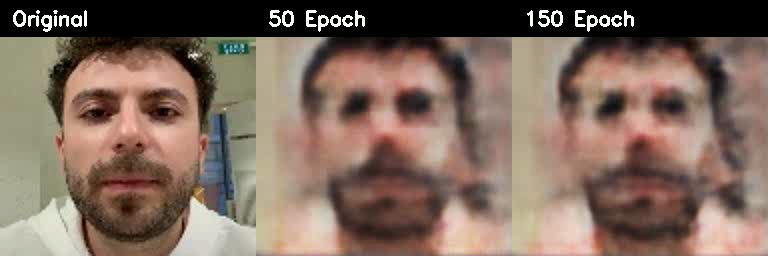
\includegraphics[width=\linewidth, height=1.9cm, keepaspectratio]{ae_vid_comp_A_to_B.png} \\
            \vspace{0.05cm}
            \scriptsize \textit{Comparison A $\to$ B (Input $\mid$ 50ep $\mid$ 150ep)}

            \vspace{0.08cm}
            \href{videos/deepfake_150_A_to_B.mp4}{\tiny \underline{\textcolor{primaryNavy}{[deepfake\_150\_A\_to\_B.mp4]}}} \quad
            \href{videos/comparison_A_to_B.mp4}{\tiny \underline{\textcolor{primaryNavy}{[comparison\_A\_to\_B.mp4]}}}
        \end{column}
    \end{columns}
\end{frame}

% --- Slide 3: Observations & Failure Analysis ---
\begin{frame}{Custom Autoencoder: Observations \& Failure Analysis}
    \begin{columns}[c]
        \begin{column}{0.50\textwidth}
            \begin{alertblock}{Observations \& Hypotheses}
                \small
                \begin{itemize}
                    \item \textbf{Observation.} The swap failed in this run: the A $\to$ B face did not look like Person B, and B $\to$ A did not look like Person A.
                    \item \textbf{Observation.} The 50 and 150 epoch videos showed no clear improvement.
                    \item \textbf{Hypothesis.} Pixel-wise MSE may train the model to recreate the original face, not to swap it.
                    \item \textbf{Hypothesis.} 238 training images may be too few.
                    \item \textbf{Hypothesis.} The shared latent code may entangle identity with pose and expression.
                    \item \textbf{Status.} We did not test these causes separately. The loss still fell slowly in the last five recorded epochs, so five points alone do not prove steady convergence.
                \end{itemize}
            \end{alertblock}
        \end{column}

        \begin{column}{0.46\textwidth}
            \centering
            \textbf{\footnotesize Triplet Video Comparison Frame}

            \vspace{0.15cm}
            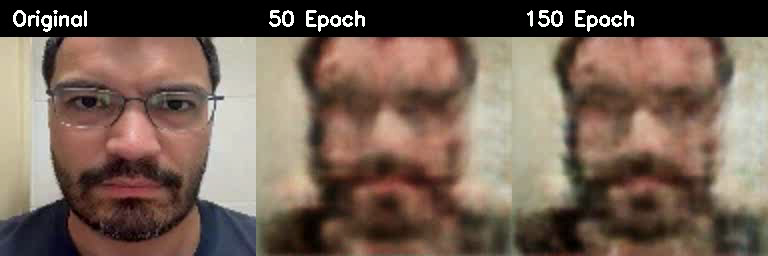
\includegraphics[width=\linewidth, height=2.1cm, keepaspectratio]{ae_vid_comp_B_to_A.png} \\
            \vspace{0.05cm}
            \scriptsize \textit{Comparison B $\to$ A (Input $\mid$ 50ep $\mid$ 150ep)}

            \vspace{0.1cm}
            \href{videos/comparison_B_to_A.mp4}{\scriptsize \underline{\textcolor{primaryNavy}{[comparison\_B\_to\_A.mp4]}}}

            \vspace{0.15cm}
            \begin{block}{Key Takeaway}
                \scriptsize
                Possible cause: the shared latent code entangled identity with facial pose and expression. This was not tested separately.
            \end{block}
        \end{column}
    \end{columns}
\end{frame}


% --- Slide 4: Pretrained Models Benchmark (FaceFusion) ---
\begin{frame}{Benchmarking Pretrained Models (FaceFusion)}
    \begin{columns}[c]
        \begin{column}{0.48\textwidth}
            \small
            \textbf{Inference Setup}
            \begin{itemize}
                \footnotesize
                \item Tested 3 pretrained models in FaceFusion (no retraining).
                \item Source face gives identity; target video gives movement.
            \end{itemize}

            \vspace{0.08cm}
            \centering
            \footnotesize
            \begin{tabular}{lccc}
                \toprule
                \textbf{Model} & \textbf{Output Size} & \textbf{Frames} & \textbf{Duration} \\
                \midrule
                HyperSwap 1A & $576 \times 1024$ & 576 & $\sim$19.25\,s \\
                InSwapper 128 & $576 \times 1024$ & 576 & $\sim$19.25\,s \\
                SimSwap 256 & $576 \times 1024$ & 576 & $\sim$19.25\,s \\
                \bottomrule
            \end{tabular}

            \vspace{0.12cm}
            \raggedright
            \small \textbf{Visual Comparison}
            \begin{itemize}
                \footnotesize
                \item \textbf{HyperSwap \& InSwapper:} Fairly natural and consistent.
                \item \textbf{SimSwap:} Followed motion, but showed artifacts around eyes and skin texture.
            \end{itemize}
        \end{column}

        \begin{column}{0.48\textwidth}
            \centering
            \begin{columns}[c]
                \begin{column}{0.31\linewidth}
                    \centering
                    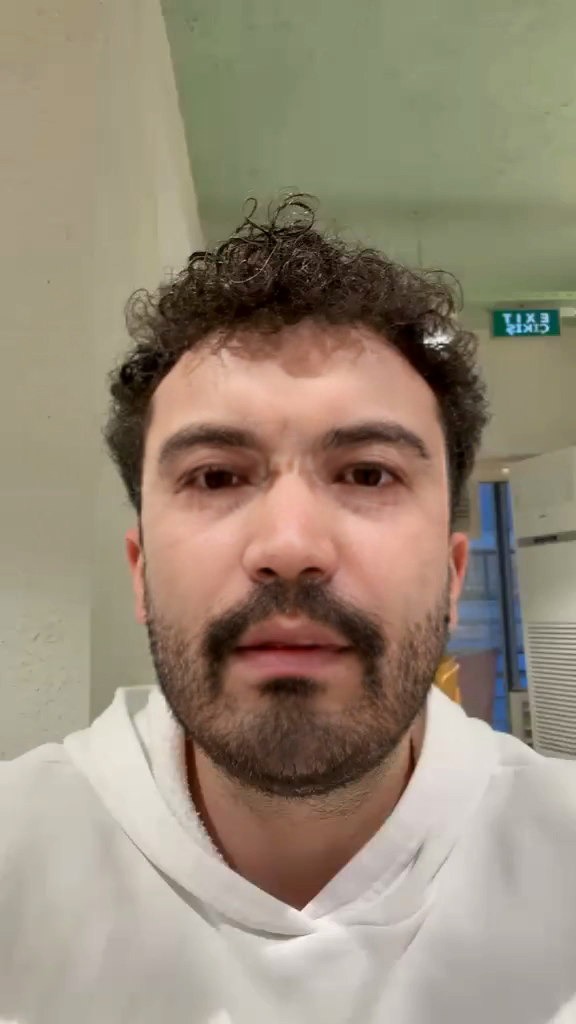
\includegraphics[height=2.8cm, keepaspectratio]{ae_vid_ff_hyperswap.png} \\
                    \tiny \textbf{HyperSwap 1A} \\
                    \href{videos/hyperswap_1a_256.mp4}{\tiny \underline{\textcolor{primaryNavy}{[hyperswap\_1a\_256.mp4]}}}
                \end{column}
                \begin{column}{0.31\linewidth}
                    \centering
                    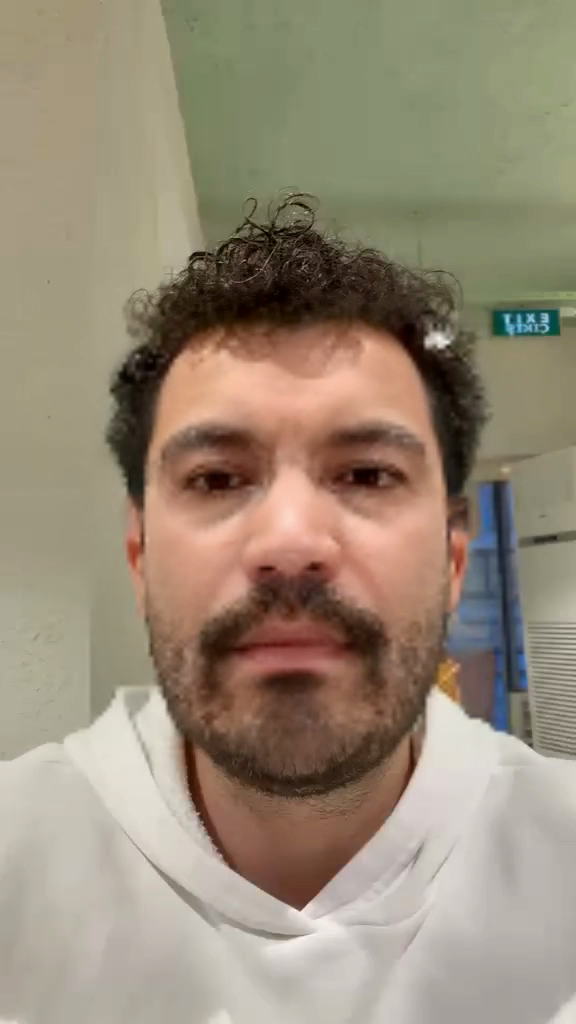
\includegraphics[height=2.8cm, keepaspectratio]{ae_vid_ff_inswapper.png} \\
                    \tiny \textbf{InSwapper 128} \\
                    \href{videos/inswapper_128.mp4}{\tiny \underline{\textcolor{primaryNavy}{[inswapper\_128.mp4]}}}
                \end{column}
                \begin{column}{0.31\linewidth}
                    \centering
                    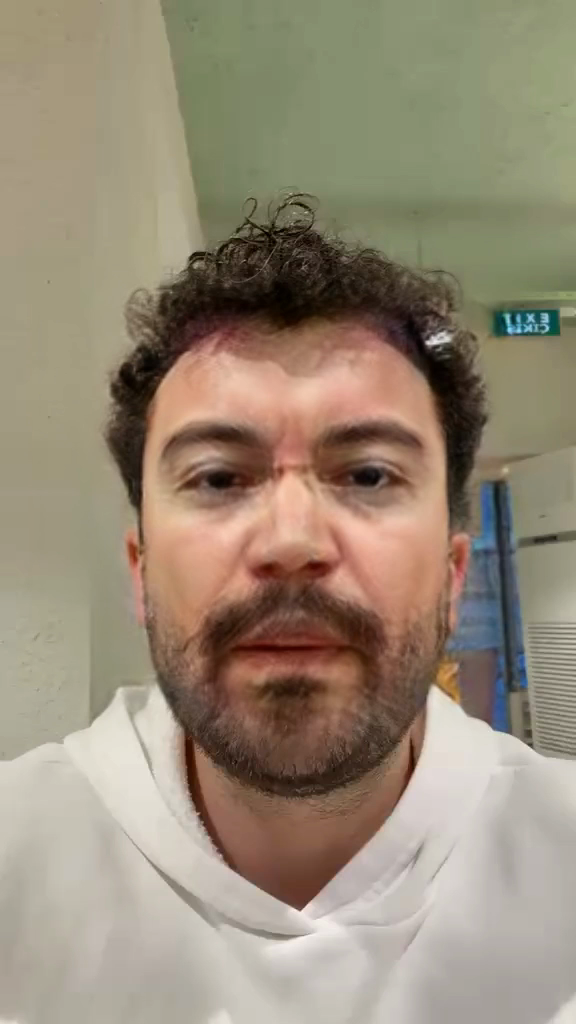
\includegraphics[height=2.8cm, keepaspectratio]{ae_vid_ff_simswap.png} \\
                    \tiny \textbf{SimSwap 256} \\
                    \href{videos/simswap_256.mp4}{\tiny \underline{\textcolor{primaryNavy}{[simswap\_256.mp4]}}}
                \end{column}
            \end{columns}

            \vspace{0.12cm}
            \scriptsize \textit{First frames: Erdem on Yusuf swaps}
        \end{column}
    \end{columns}
\end{frame}


% --- Slide 5: Evaluation & Lessons Learned ---
\begin{frame}{Autoencoders: Evaluation \& Lessons Learned}
    \begin{columns}[T]
        \begin{column}{0.48\textwidth}
            \begin{block}{Overall Evaluation}
                \small
                \begin{itemize}
                    \item Training our own autoencoder was not successful for face swapping.
                    \item FaceFusion pretrained models gave much more promising results.
                    \item Showed the importance of using models designed specifically for face swapping.
                    \item Having only 100 images for Person A and 138 for Person B was a major limitation.
                \end{itemize}
            \end{block}
        \end{column}

        \begin{column}{0.48\textwidth}
            \begin{exampleblock}{Lessons Learned (Erdem's Takeaways)}
                \small
                \begin{itemize}
                    \item \textbf{Low loss $\neq$ usable result:} The model got better at reconstructing faces, but not at swapping them. Another 100 epochs did not fix this.
                    \item \textbf{Beyond running tools:} Building our own model helped us understand preprocessing, training, and evaluation hands-on.
                    \item Pretrained models helped us compare how task-specific designs improve the result.
                \end{itemize}
            \end{exampleblock}
        \end{column}
    \end{columns}
\end{frame}



% -------------------------------------------------------------
% 3. Method 2: GANs & First Order Motion Model (Detailed)
% -------------------------------------------------------------
\section{Method 2: GANs \& FOMM}

% --- Slide 1: Standard GAN ---
\begin{frame}{Standard GAN Architecture}
    \begin{columns}[c]
        \begin{column}{0.48\textwidth}
            \textbf{How GANs Work (Goodfellow et al., 2014)}
            \begin{itemize}
                \item Two neural networks competing against each other in an adversarial setup:
                \item \textbf{Generator ($G$):} Takes a random noise vector $\mathbf{z}$ and learns to synthesize realistic facial images.
                \item \textbf{Discriminator ($D$):} Evaluates images and classifies them as real (from dataset) or fake (from $G$).
                \item \textbf{Adversarial training:} Through gradient feedback, $G$ progressively captures fine details and photorealistic textures.
            \end{itemize}
        \end{column}

        \begin{column}{0.50\textwidth}
            \centering
            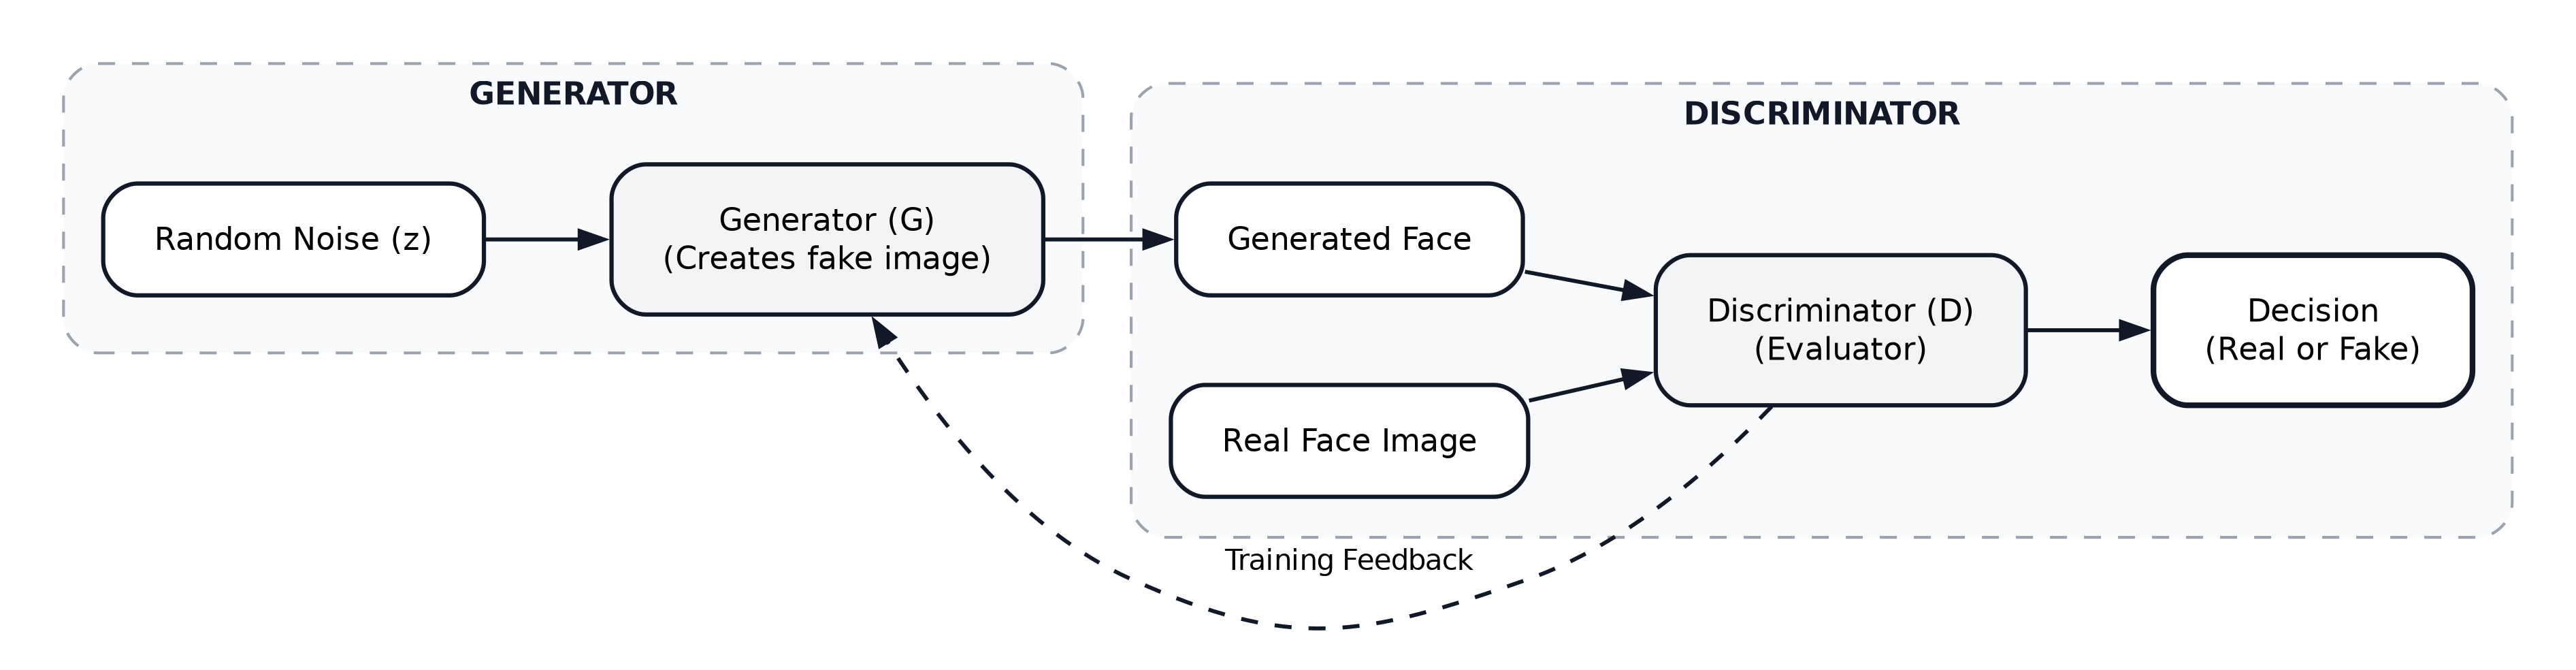
\includegraphics[width=\linewidth, height=4.2cm, keepaspectratio]{diagram_standard_gan.png}
        \end{column}
    \end{columns}
\end{frame}

% --- Slide 2: Why Standard GANs Fail ---
\begin{frame}{The Controllability Issue in Vanilla GANs}
    \begin{columns}[c]
        \begin{column}{0.50\textwidth}
            \begin{block}{Why Unconditional GANs Fall Short}
                \small
                \begin{itemize}
                    \item Generates arbitrary faces from random noise $\mathbf{z}$.
                    \item Identity, pose, and emotion are entangled in latent space.
                    \item Cannot say: \textit{"keep Person A, copy Person B's expression"}.
                \end{itemize}
            \end{block}
            
            \begin{block}{What Face Reenactment Requires}
                \small
                \begin{itemize}
                    \item \textbf{Identity conditioning:} Appearance anchored strictly to source portrait $S$.
                    \item \textbf{Motion conditioning:} Facial dynamics driven frame-by-frame by driving video $D$.
                \end{itemize}
            \end{block}
        \end{column}

        \begin{column}{0.48\textwidth}
            \centering
            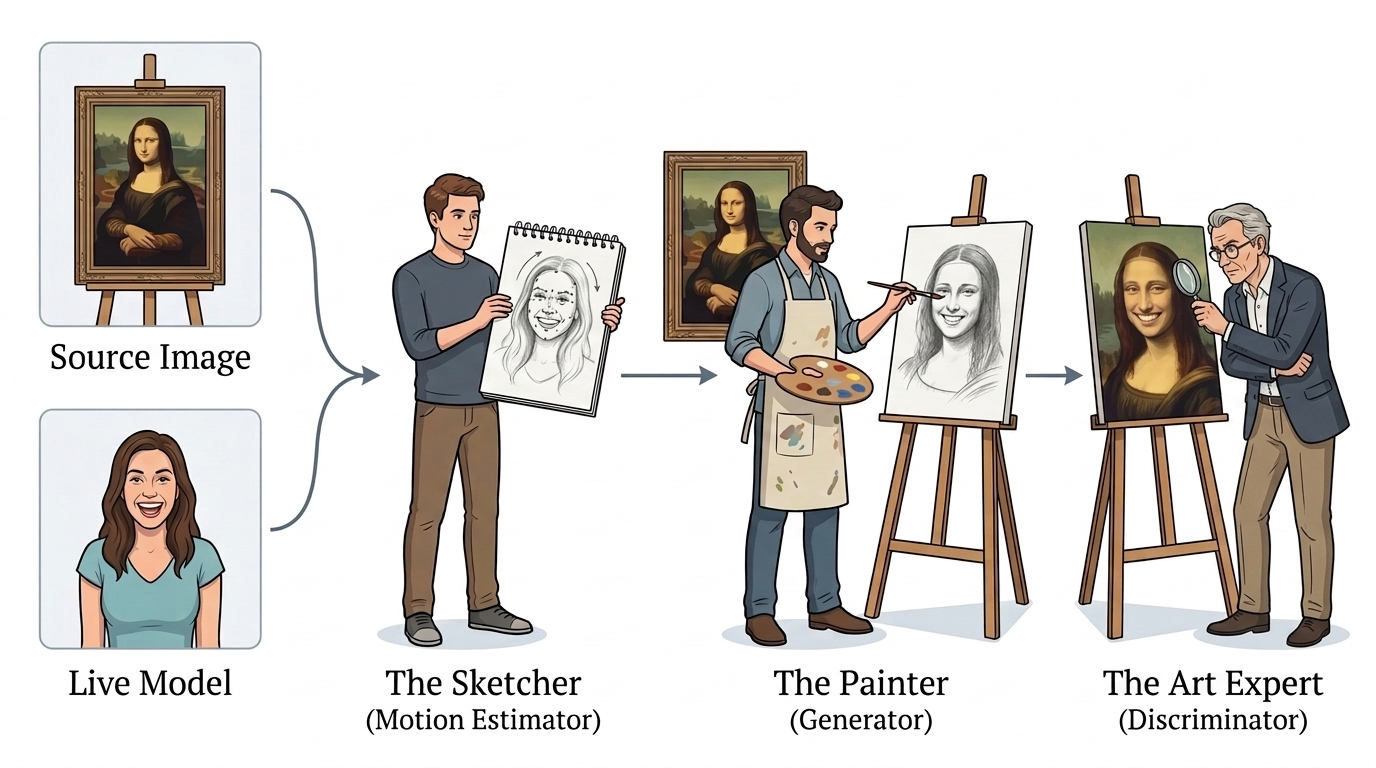
\includegraphics[width=\linewidth, keepaspectratio]{ressam_dedektif_analoji.png}
        \end{column}
    \end{columns}
\end{frame}

% --- Slide 1: FOMM Overview ---
\begin{frame}{First Order Motion Model (Siarohin et al., NeurIPS 2019)}
    \begin{columns}[c]
        \begin{column}{0.54\textwidth}
            \textbf{Core Innovations}
            \begin{itemize}
                \item \textbf{No Pretrained Landmarks:} Doesn't need 68 facial landmark detectors or 3D face models (3DMM).
                \item \textbf{Self-Supervised:} Learns keypoints automatically from raw video pairs.
                \item \textbf{Appearance / Motion Decoupling:} Appearance comes from source $S$; motion comes from driving $D$.
                \item \textbf{Generalizes Across Domains:} Works on human faces, bodies (Tai-Chi), and animals.
            \end{itemize}
        \end{column}

        \begin{column}{0.44\textwidth}
            \centering
            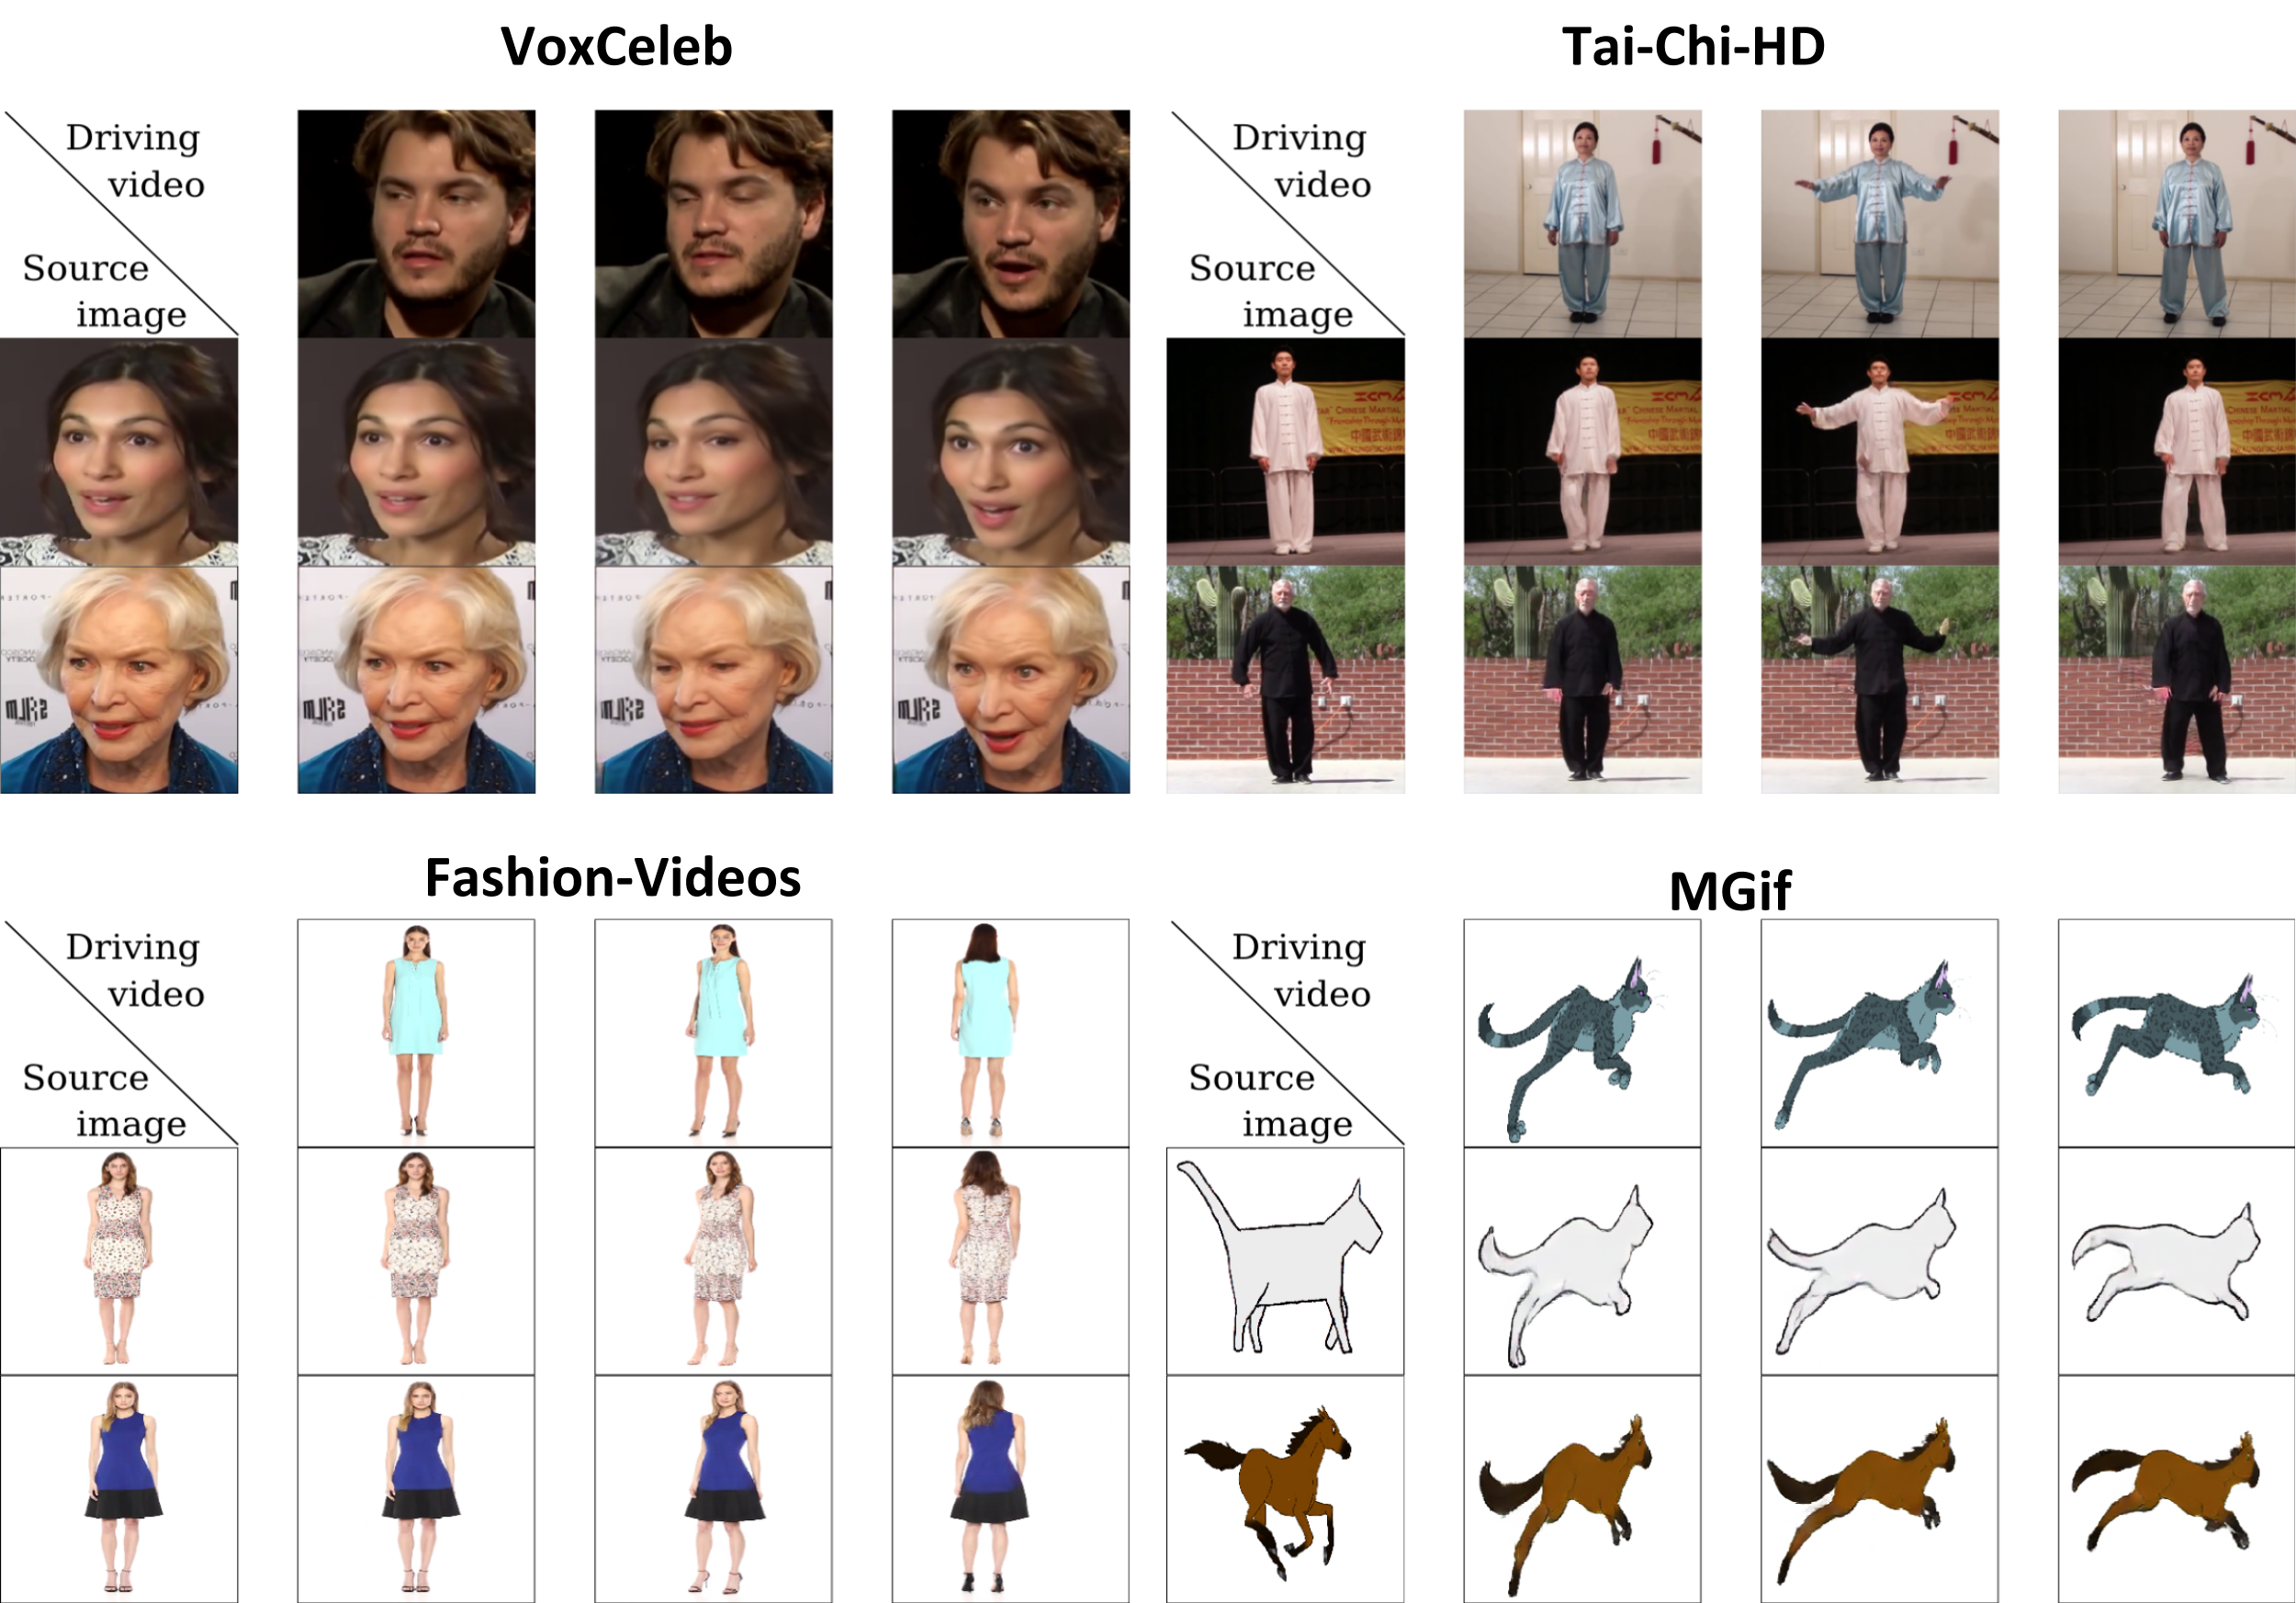
\includegraphics[width=\linewidth, height=3.8cm, keepaspectratio]{fomm_teaser.png}
            \vspace{0.15cm}
            
            \scriptsize \textit{FOMM teaser: VoxCeleb, Tai-Chi, Fashion (Siarohin et al., 2019).}
        \end{column}
    \end{columns}
\end{frame}

% --- Slide 2: Motion Representation: 0th vs 1st Order ---
\begin{frame}{Motion Representation: 0th-Order vs. 1st-Order Motion}
    \begin{columns}[c]
        \begin{column}{0.48\textwidth}
            \textbf{Motion Representation}
            \begin{itemize}
                \item \textbf{0th-Order (Translation Only):}
                \begin{itemize}
                    \item Moves points in 2D space $(x, y)$.
                    \item Cannot stretch skin; movement looks stiff and robotic.
                \end{itemize}
                \vspace{0.25cm}
                \item \textbf{1st-Order (FOMM):}
                \begin{itemize}
                    \item Tracks deformation around each point.
                    \item Captures rotation (head tilts), scale (mouth opening), and shear (skin stretch).
                \end{itemize}
            \end{itemize}
        \end{column}

        \begin{column}{0.50\textwidth}
            \centering
            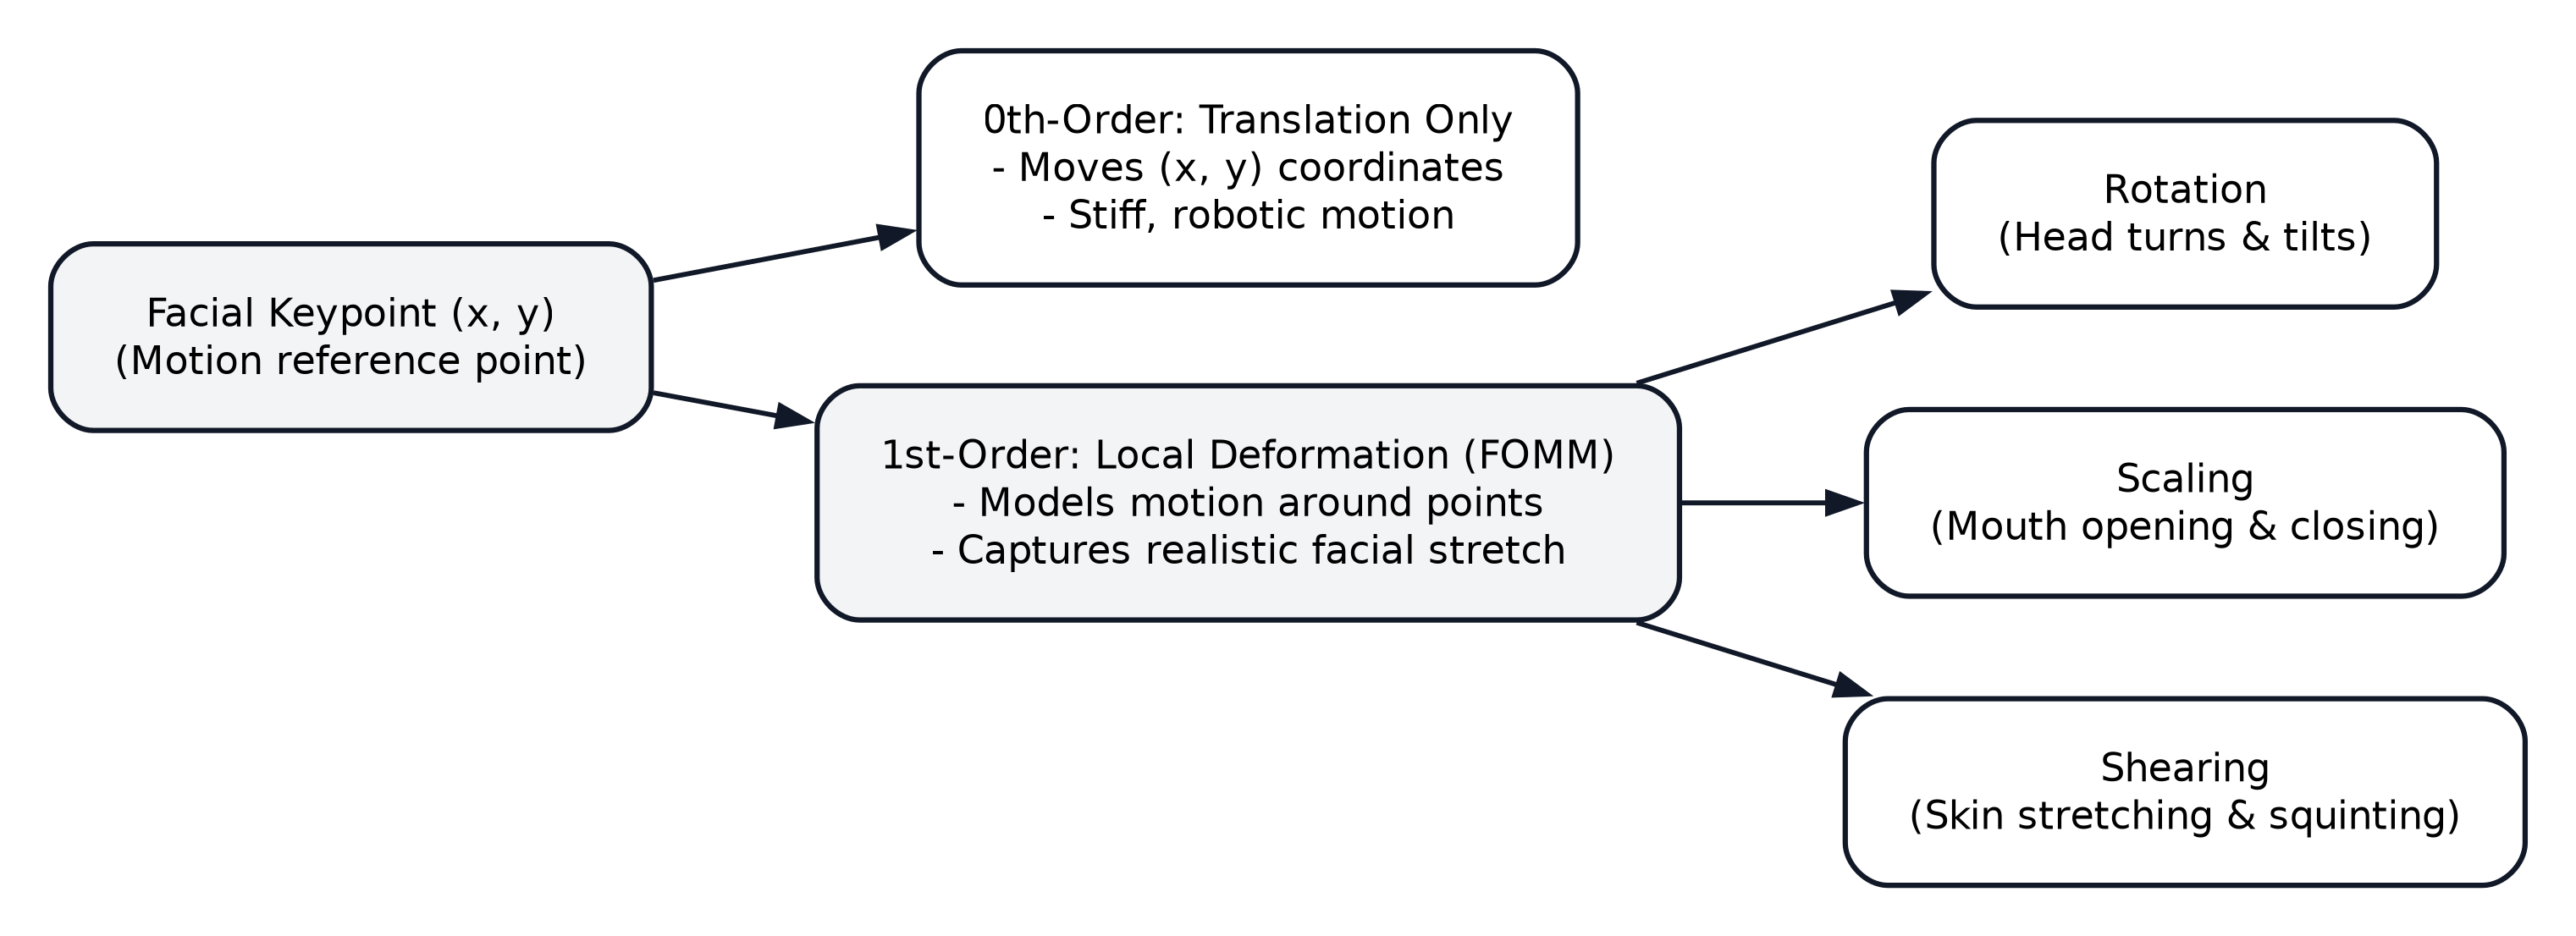
\includegraphics[width=\linewidth, height=4.2cm, keepaspectratio]{diagram_facial_motion_order.png}
        \end{column}
    \end{columns}
\end{frame}

% --- Slide 3: The FOMM Pipeline & Core Components ---
\begin{frame}{FOMM Architectural Pipeline}
    \begin{center}
        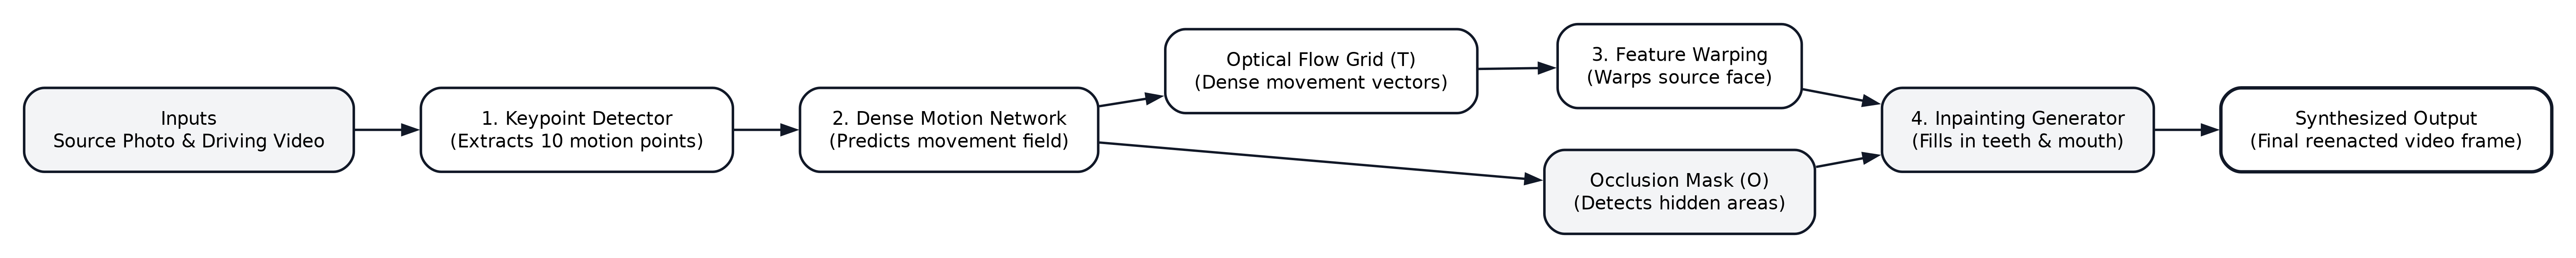
\includegraphics[width=0.96\linewidth, height=3.0cm, keepaspectratio]{diagram_fomm_pipeline.png}
    \end{center}

    \vspace{0.15cm}

    \begin{columns}[T]
        \begin{column}{0.32\textwidth}
            \begin{block}{1. Keypoint Detector}
                \scriptsize Hourglass network detects $K=10$ unsupervised keypoints and Jacobians.
            \end{block}
        \end{column}
        \begin{column}{0.32\textwidth}
            \begin{block}{2. Dense Motion Network}
                \scriptsize Converts sparse points into optical flow ($T$) and an occlusion mask ($O$).
            \end{block}
        \end{column}
        \begin{column}{0.32\textwidth}
            \begin{block}{3. Inpainting Generator}
                \scriptsize Warps source features using $T$ and inpaints occluded areas ($O \approx 0$).
            \end{block}
        \end{column}
    \end{columns}
\end{frame}

% --- Slide 1: Self-Occlusion & The Need for Inpainting ---
\begin{frame}{Self-Occlusion \& Inpainting}
    \begin{columns}[c]
        \begin{column}{0.48\textwidth}
            \begin{block}{The Problem}
                \small
                \begin{itemize}
                    \item Turning head or opening mouth reveals parts not visible in source $S$ (teeth, tongue, cheeks).
                    \item Pure warping has no pixels to sample from $\to$ stretches or leaves black holes.
                \end{itemize}
            \end{block}

            \begin{block}{The Fix}
                \small
                \begin{itemize}
                    \item \textbf{Occlusion Mask ($O$):} Flags missing pixels ($O \approx 0$).
                    \item \textbf{Inpainting:} Generator fills missing pixels using facial patterns learned during training.
                \end{itemize}
            \end{block}
        \end{column}

        \begin{column}{0.50\textwidth}
            \centering
            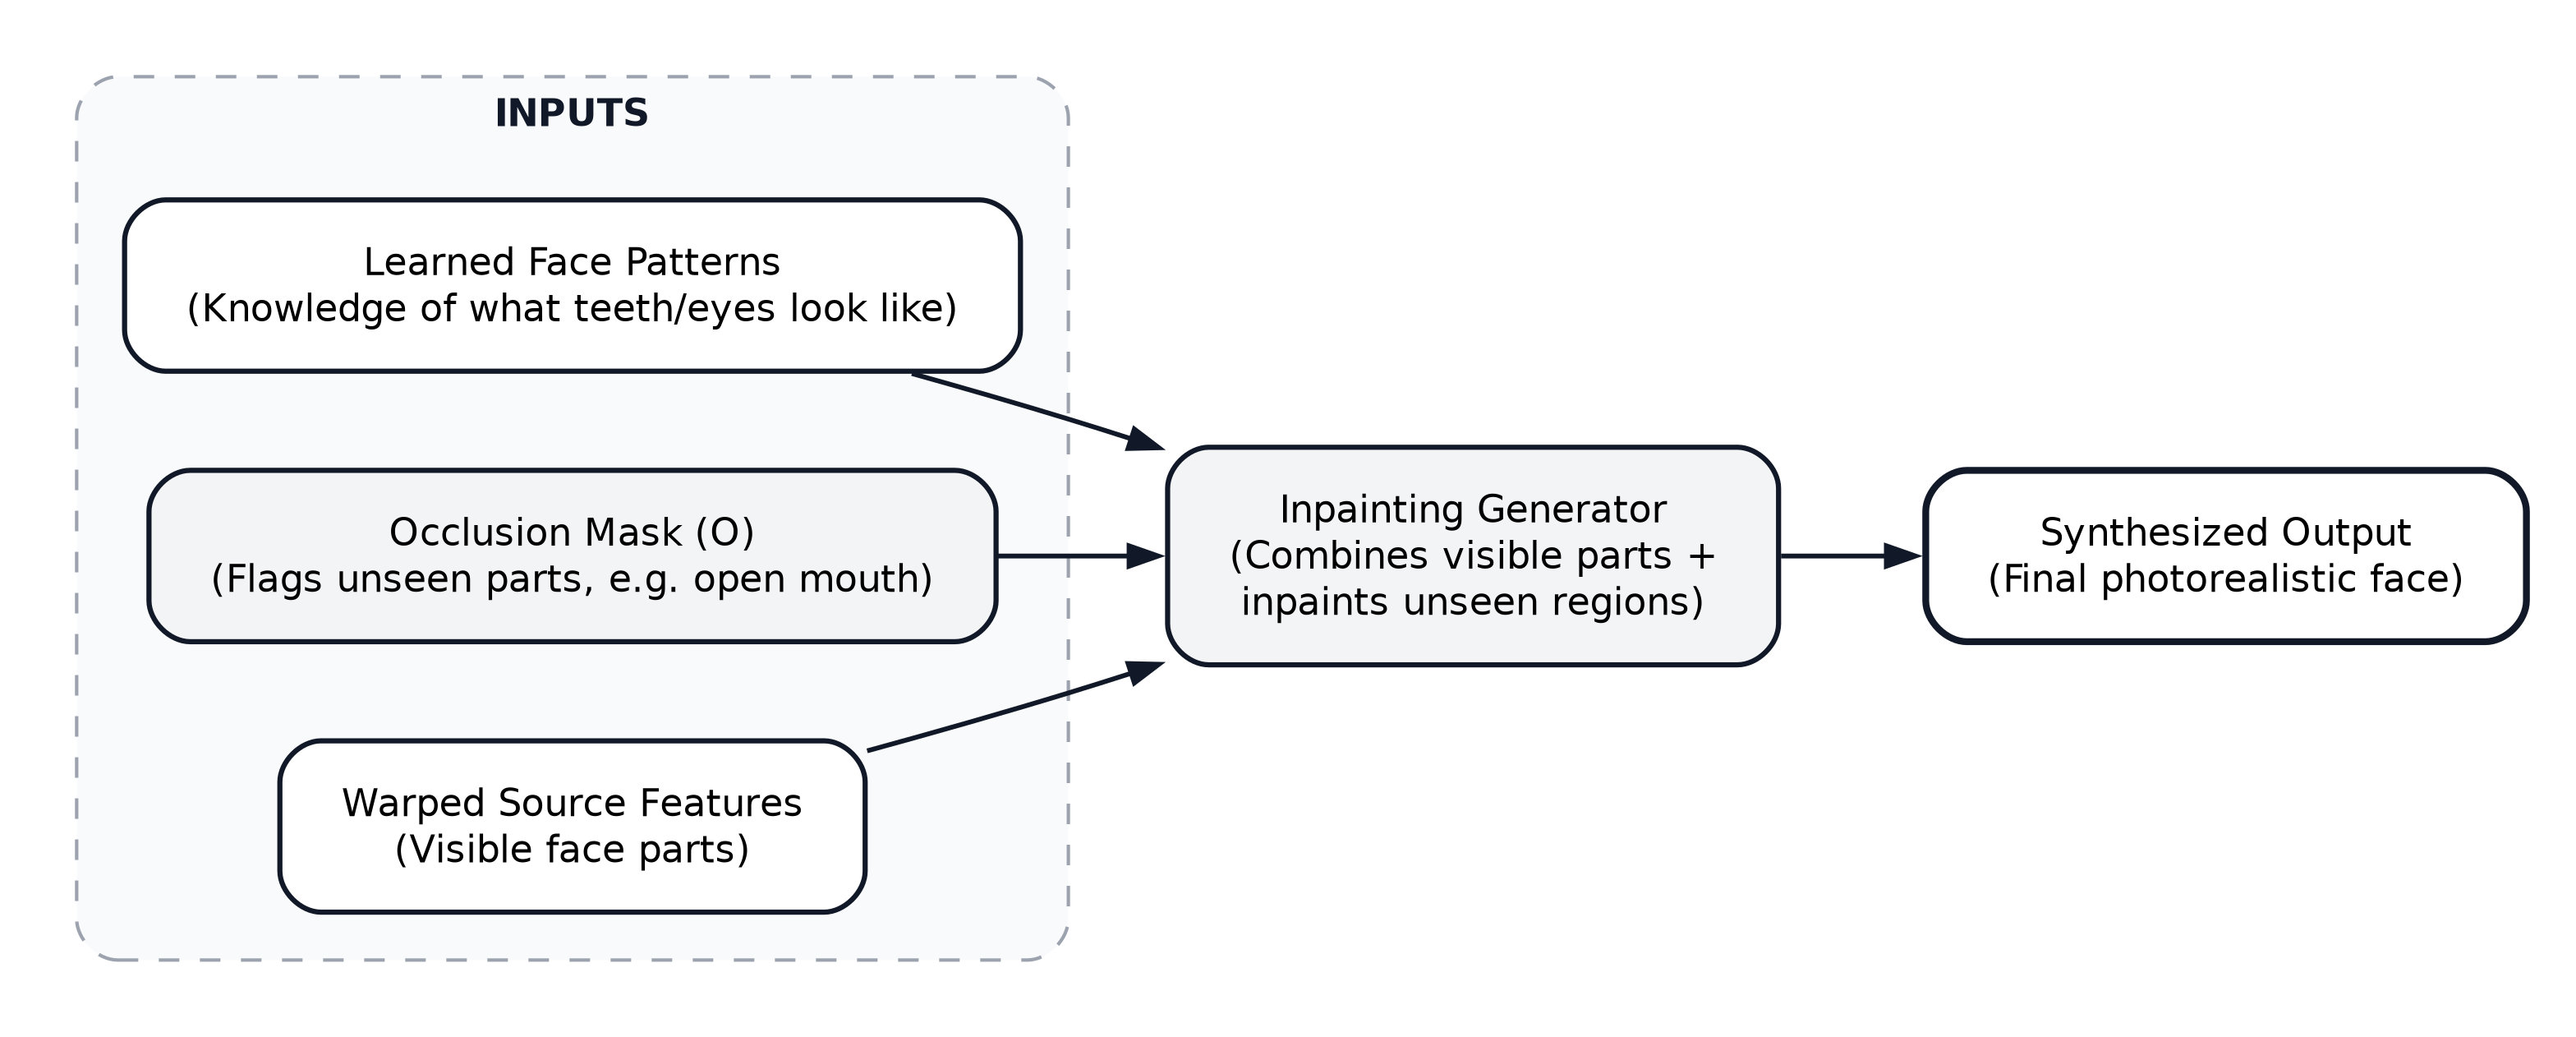
\includegraphics[width=\linewidth, height=4.2cm, keepaspectratio]{diagram_occlusion_inpainting.png}
        \end{column}
    \end{columns}
\end{frame}

% --- Slide 2: Visual Proof of Pipeline Execution (Intermediate Stages) ---
\begin{frame}{Pipeline Verification: Intermediate Stages}
    \begin{center}
        \small \textbf{5 Intermediate Stages Extracted During Local Inference}
    \end{center}
    
    \vspace{-0.1cm}
    \begin{center}
        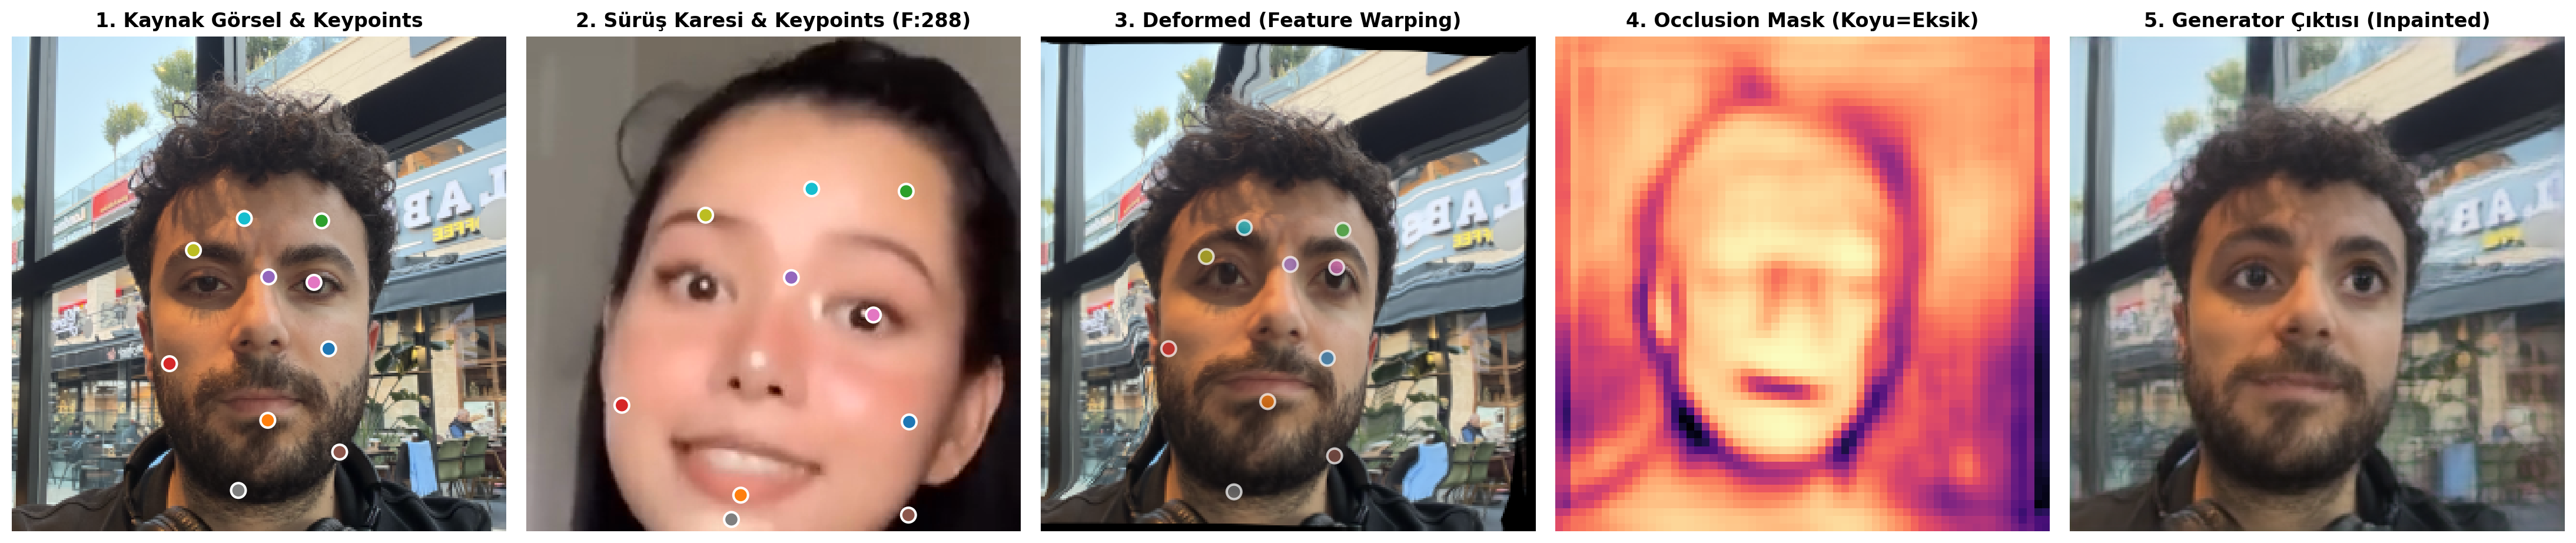
\includegraphics[width=0.96\linewidth, height=3.5cm, keepaspectratio]{ara_asamalar_gorsellestirme.png}
    \end{center}
    \vspace{-0.1cm}
    
    \begin{columns}[T]
        \begin{column}{0.19\textwidth}
            \centering \scriptsize \textbf{1. Source Points}\\
            $S$ reference keypoints
        \end{column}
        \begin{column}{0.19\textwidth}
            \centering \scriptsize \textbf{2. Driving Points}\\
            $D$ tracking points
        \end{column}
        \begin{column}{0.19\textwidth}
            \centering \scriptsize \textbf{3. Warped Frame}\\
            Flow-deformed source
        \end{column}
        \begin{column}{0.19\textwidth}
            \centering \scriptsize \textbf{4. Occlusion Mask}\\
            Dark = missing regions
        \end{column}
        \begin{column}{0.19\textwidth}
            \centering \scriptsize \textbf{5. Inpainted Result}\\
            Synthesized output
        \end{column}
    \end{columns}
\end{frame}

% --- Slide 1: Inference Pipeline Pseudocode ---
\begin{frame}[fragile]{Inference Pipeline: Python Pseudocode}
    \begin{columns}[T]
        \begin{column}{0.56\textwidth}
            \begin{block}{Frame-by-Frame Execution Loop}
                \scriptsize
\begin{verbatim}
# 1. Extract reference keypoints from source portrait
kp_source = keypoint_detector(source_image)

# 2. Iterate through driving video frames
for frame_d in driving_video:
    # Step 1: Motion tracking
    kp_driving = keypoint_detector(frame_d)

    # Step 2: Dense motion & occlusion estimation
    flow, occ = dense_motion_net(kp_source, kp_driving)

    # Step 3: Flow warping & inpainting
    out_frame = generator(source_image, flow, occ)

    yield out_frame
\end{verbatim}
            \end{block}
        \end{column}

        \begin{column}{0.41\textwidth}
            \small \textbf{Core Modules}
            \begin{itemize}
                \footnotesize
                \item \texttt{keypoint\_detector}: Extracts 10 unsupervised keypoints.
                \item \texttt{dense\_motion\_net}: Computes optical flow and occlusion mask.
                \item \texttt{generator}: Warps source pixels and inpaints mouth/teeth.
            \end{itemize}

            \vspace{0.1cm}
            \begin{block}{Architectural Property}
                \scriptsize \textbf{No Recurrence:} The loop carries no hidden state across frames ($t \to t+1$).
            \end{block}
        \end{column}
    \end{columns}
\end{frame}

% --- Slide 2: Side-by-Side Results & External Video Links ---
\begin{frame}{Experimental Results: Bella Poarch Benchmark}
    \begin{center}
        \small \textbf{Triplets: [Source Portrait $\mid$ Driving Frame $\mid$ Synthesized Result]}
    \end{center}

    \vspace{0.05cm}
    \begin{columns}[c]
        \begin{column}{0.32\textwidth}
            \centering
            
\includegraphics[width=\linewidth, height=2.1cm, keepaspectratio]{bella_comparison_f30.png}
            \vspace{0.05cm}
            
            \scriptsize \textit{Frame 30 (1.0s): Head Tilt}
        \end{column}
        \begin{column}{0.32\textwidth}
            \centering
            
\includegraphics[width=\linewidth, height=2.1cm, keepaspectratio]{bella_comparison_f286.png}
            \vspace{0.05cm}
            
            \scriptsize \textit{Frame 286 (9.5s): Smile \& Squint}
        \end{column}
        \begin{column}{0.32\textwidth}
            \centering
            
\includegraphics[width=\linewidth, height=2.1cm, keepaspectratio]{bella_comparison_f20.png}
            \vspace{0.05cm}
            
            \scriptsize \textit{Frame 20 (0.7s): Mouth Opening}
        \end{column}
    \end{columns}

    \vspace{0.15cm}
    
    \begin{block}{Demo Video Link}
        \scriptsize
        \begin{itemize}
            \item \textbf{3$\times$3 Multi-Subject Comparison Video (All Members):} \href{https://www.youtube.com/shorts/1zLsU1j765I}{\underline{\textcolor{primaryNavy}{Watch Online (External Link)}}}
        \end{itemize}
    \end{block}
\end{frame}

% --- Slide 1: Hypothesis & Setup for Edge Case ---
\begin{frame}{Failure Mode Experiment: Dental Braces}
    \begin{columns}[T]
        \begin{column}{0.50\textwidth}
            \begin{block}{Experiment Setup}
                \small
                \begin{itemize}
                    \item \textbf{Test Idea:} How does FOMM handle rare facial features absent from training data?
                    \item \textbf{Subject:} Source portrait with metallic dental braces (\texttt{bella\_poarch\_dis\_teli}).
                    \item \textbf{Driving Motion:} Sequences from subtle head tilt to closed mouth, ending in a wide squinting smile.
                \end{itemize}
            \end{block}
        \end{column}

        \begin{column}{0.48\textwidth}
            \begin{block}{Hypothesis}
                \small
                \begin{itemize}
                    \item VoxCeleb training data has virtually zero faces with dental braces.
                    \item \textbf{Warping Regime ($O \approx 1$):} Optical flow copies real source pixels $\to$ braces preserved.
                    \item \textbf{Inpainting Regime ($O \approx 0$):} Under extreme deformation, model flags teeth as occluded and synthesizes them.
                    \item \textbf{Prediction:} Inpainting will sample dataset average and erase braces.
                \end{itemize}
            \end{block}
        \end{column}
    \end{columns}
\end{frame}

% --- Slide 2: Visual Evidence of Failure Mode (3x3 Grid) ---
\begin{frame}{Failure Mode: Vanishing Dental Braces}
    \begin{columns}[c]
        \begin{column}{0.54\textwidth}
            \centering
            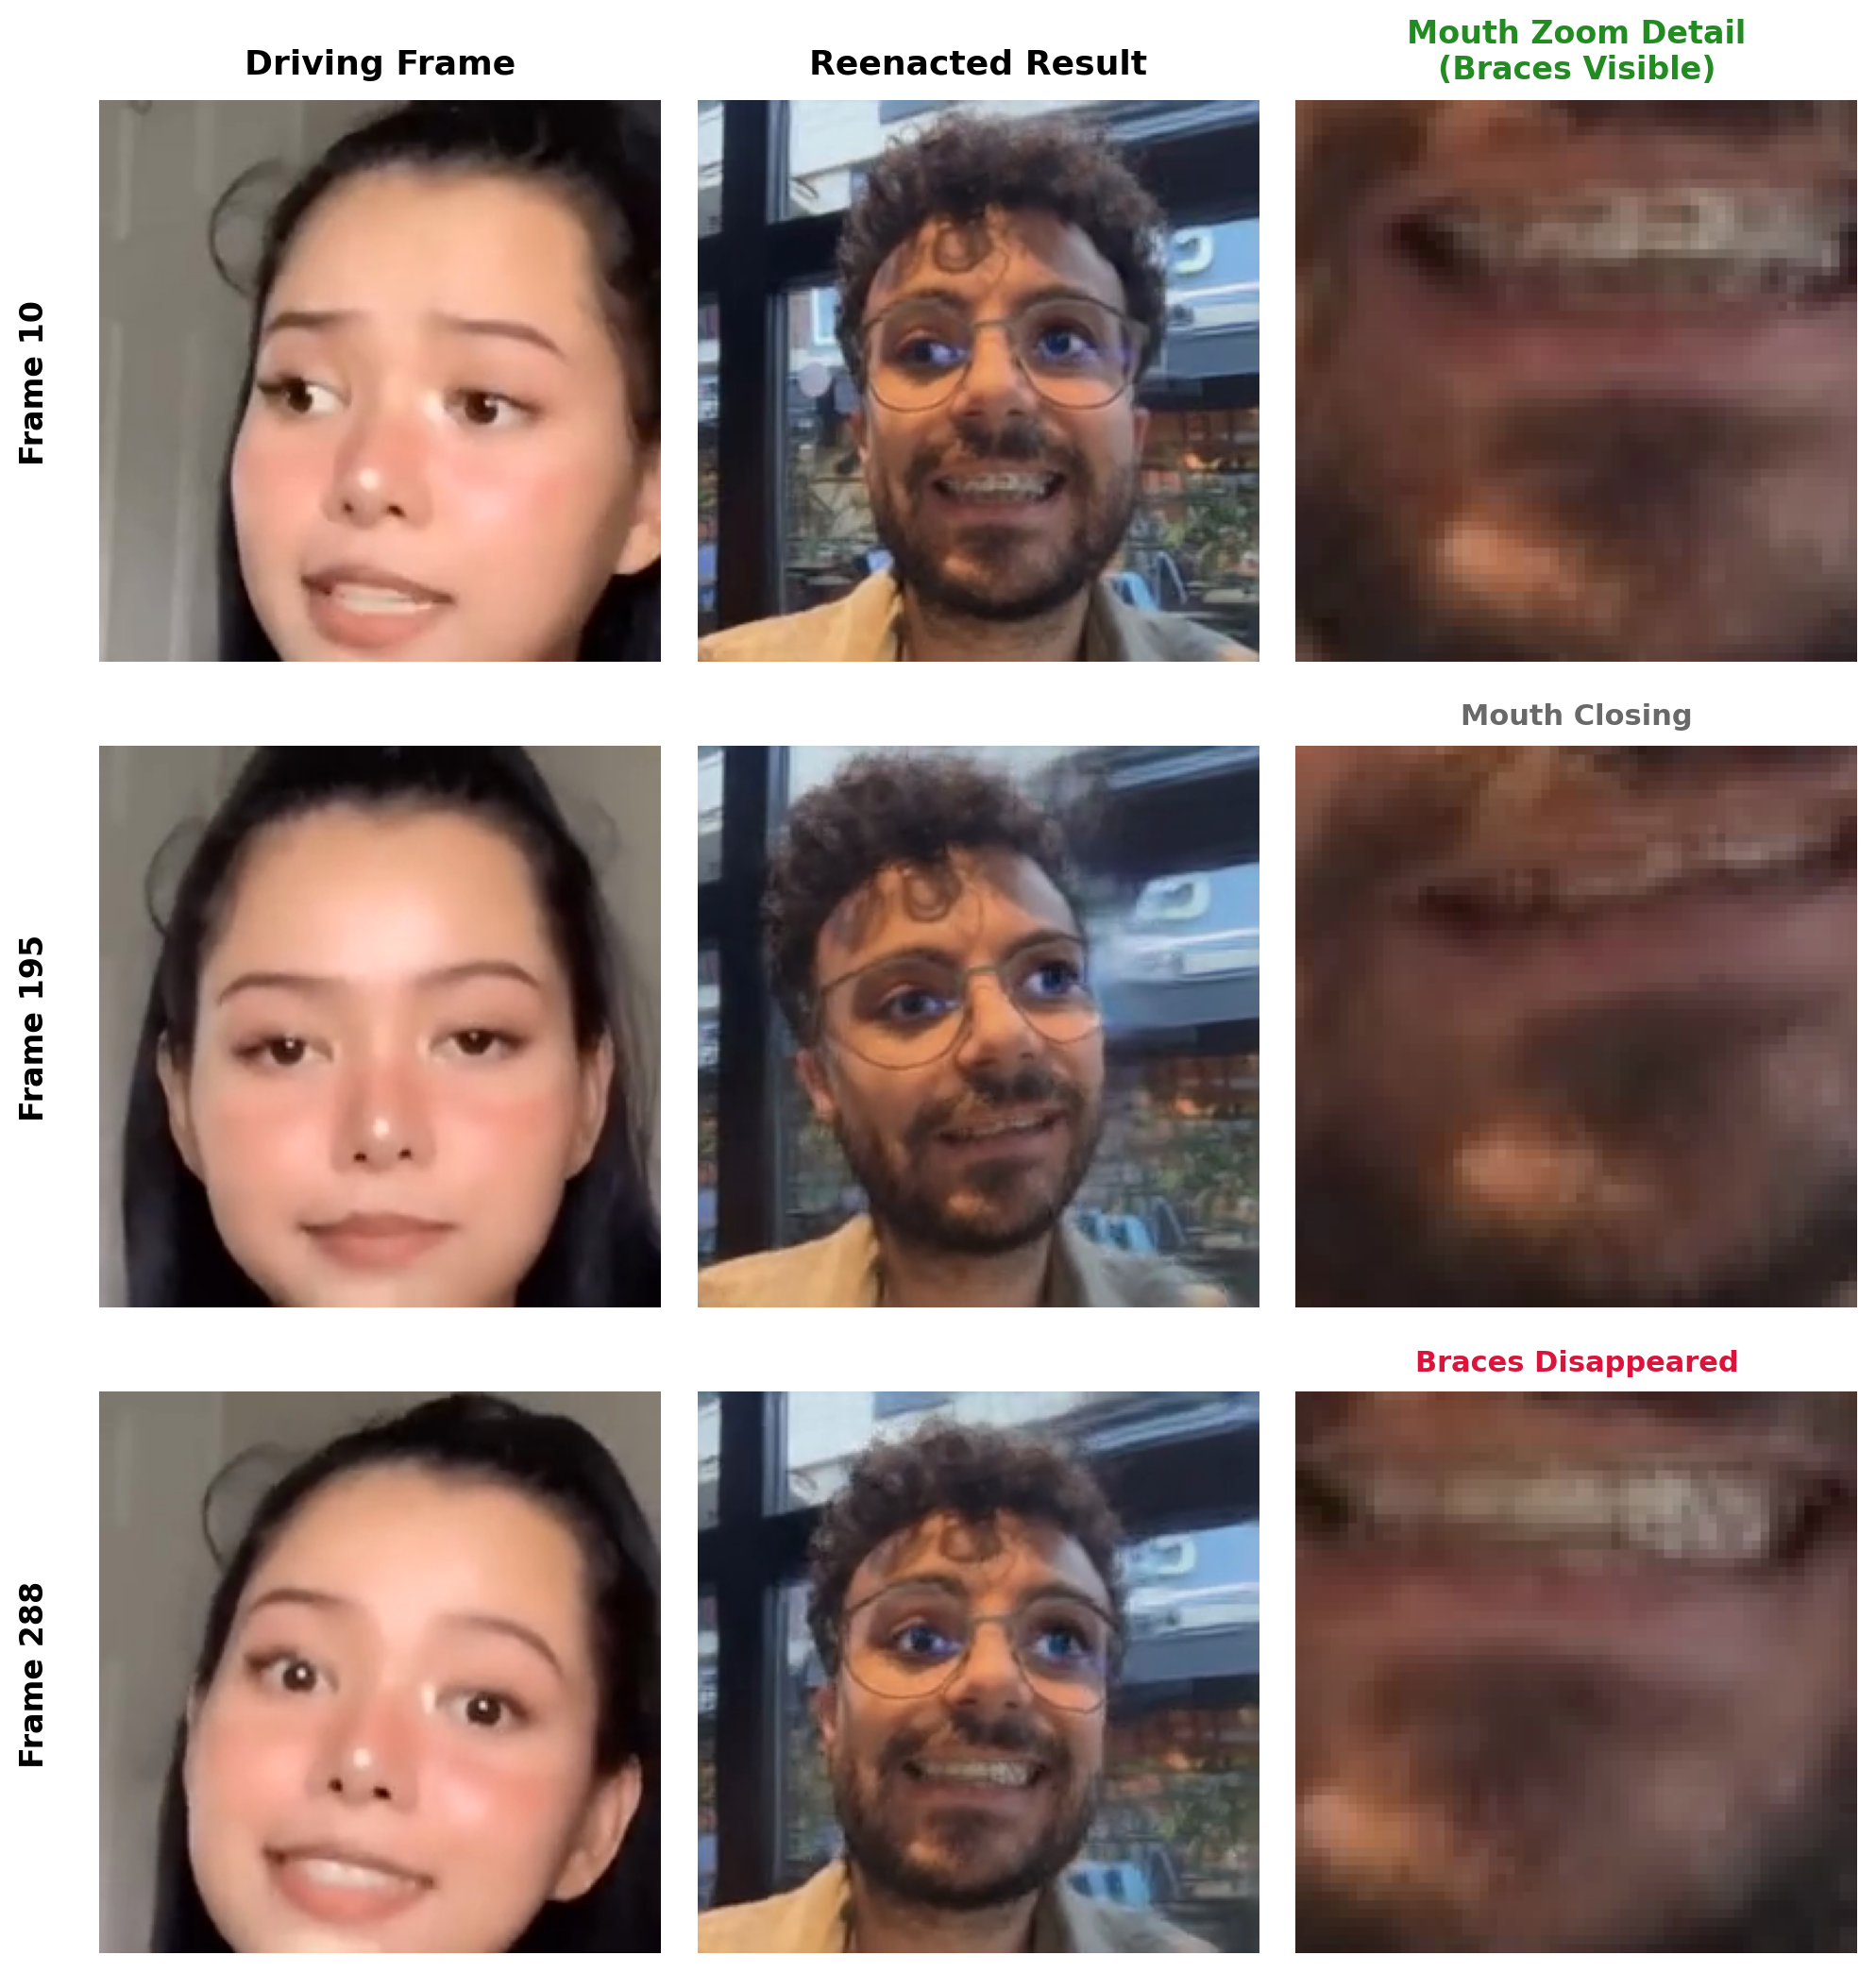
\includegraphics[width=\linewidth, height=5.2cm, keepaspectratio]{dis_teli_kaybolma_analizi.png}
            \vspace{0.05cm}
            
            \scriptsize \textit{Frame 10 (top), Frame 195 (middle), Frame 288 (bottom).}
        \end{column}

        \begin{column}{0.44\textwidth}
            \textbf{Observation Across Frames:}
            \begin{itemize}
                \item \textbf{Frame 10 (0.3s) — Warping:} Small motion offset; teeth mapped from source ($O \approx 1$). Metallic brackets intact.
                \item \textbf{Frame 195 (6.5s) — Natural Closure:} Driving mouth closes; teeth hidden behind lips.
                \item \textbf{Frame 288 (9.6s) — Inpainting Failure:} Wide squint/smile exceeds flow limits $\to$ mouth flagged as occluded ($O \approx 0$).
                \item Generator draws standard white teeth from dataset prior; \textbf{braces vanish completely}.
            \end{itemize}
        \end{column}
    \end{columns}
\end{frame}

% --- Slide 3: Root Cause Analysis & Video Links ---
\begin{frame}{Root Cause: Why Did It Fail?}
    \begin{columns}[T]
        \begin{column}{0.50\textwidth}
            \begin{block}{Technical Causes}
                \small
                \begin{enumerate}
                    \item \textbf{Stateless Generation:} Each frame is computed strictly from $(S, D_t)$. Frame 195 does not cause Frame 288's loss; Frame 288 fails due to its own extreme deformation mismatch.
                    \item \textbf{Dataset Bias in Inpainting:} When $O \approx 0$, generator ignores source pixels and samples from VoxCeleb average (normal teeth).
                    \item \textbf{Zero Identity Cache:} FOMM lacks recurrent memory to inject known identity traits into the inpainter.
                \end{enumerate}
            \end{block}
        \end{column}

        \begin{column}{0.46\textwidth}
            \begin{block}{Main Takeaway}
                \small
                \begin{itemize}
                    \item \textbf{Warping} preserves unique personal traits.
                    \item \textbf{Inpainting} pulls outputs toward dataset averages.
                    \item \textbf{Architectural Fix:} Requires 3D geometry priors or persistent identity memory.
                \end{itemize}
            \end{block}

            \vspace{0.15cm}
            \begin{block}{Braces Experiment Videos}
                \small
                \begin{itemize}
                    \item \textbf{Side-by-Side Video:} \href{https://YOUR-EXTERNAL-VIDEO-LINK-HERE}{\underline{\textcolor{primaryNavy}{Watch Online (External Link)}}}
                    \item \textbf{Reenacted Result:} \href{https://YOUR-EXTERNAL-VIDEO-LINK-HERE}{\underline{\textcolor{primaryNavy}{Watch Online (External Link)}}}
                \end{itemize}
            \end{block}
        \end{column}
    \end{columns}
\end{frame}


% -------------------------------------------------------------
% 4. Method 3: Diffusion Models (Teammate Placeholder)
% -------------------------------------------------------------
\section{Method 3: Diffusion Models}

\begin{frame}{Method 3: Diffusion Models}
    \begin{center}
        \vspace{1.5cm}
        {\Large \textbf{Diffusion Models \& Iterative Denoising}} \\
        \vspace{0.5cm}
        {\normalsize \textit{[Placeholder -- Teammate Section]}}
    \end{center}
\end{frame}


% -------------------------------------------------------------
% 5. Comparative Analysis (Team Synthesis Placeholder)
% -------------------------------------------------------------
\section{Comparative Analysis}

\begin{frame}{Comparative Analysis}
    \begin{center}
        \vspace{1.5cm}
        {\Large \textbf{Comparative Analysis}} \\
        \vspace{0.3cm}
        {\large Autoencoders vs. GANs (FOMM) vs. Diffusion Models} \\
        \vspace{0.5cm}
        {\normalsize \textit{[Placeholder -- Team Synthesis]}}
    \end{center}
\end{frame}


% -------------------------------------------------------------
% 6. Ethics & Conclusion
% -------------------------------------------------------------
\section{Ethics \& Conclusion}

% --- Slide 1: Ethics & Detection ---
\begin{frame}{Ethical Implications \& DeepFake Detection}
    \begin{columns}[T]
        \begin{column}{0.48\textwidth}
            \begin{block}{Societal Risks}
                \small
                \begin{itemize}
                    \item \textbf{Impersonation:} Reenacting individuals without their consent.
                    \item \textbf{Misinformation:} Generating fabricated videos to deceive the public.
                \end{itemize}
            \end{block}
        \end{column}

        \begin{column}{0.48\textwidth}
            \begin{block}{Detection Strategies}
                \small
                \begin{itemize}
                    \item \textbf{Blinking and rPPG:} Detection cues reported in the literature; this project ran no such test.
                    \item \textbf{Frequency artifacts:} Reported in the literature; neural upsampling leaves high-frequency noise.
                    \item \textbf{Watermarking:} A separate measure, independent of C2PA.
                    \item \textbf{C2PA:} A signed provenance and edit-history manifest, not only a capture-time stamp. It is not a deepfake detector by itself.
                \end{itemize}
            \end{block}
        \end{column}
    \end{columns}
\end{frame}

% --- Slide 2: Conclusion & Q&A ---
\begin{frame}{Conclusion}
    \begin{columns}[T]
        \begin{column}{0.55\textwidth}
            \small
            \textbf{Summary}
            \begin{itemize}
                \item \textbf{Autoencoder:} Low loss, but no identity swap; pretrained models gave better results.
                \item \textbf{FOMM:} Head turns and blinks transferred smoothly; inpainting erased rare details (braces).
                \item \textbf{Rectified Flow:} Head swap ran on a 4 GB GPU; the worst frames still jump.
                \item \textbf{Lesson:} A low loss does not mean a usable swap; use a model built for the task.
            \end{itemize}
        \end{column}

        \begin{column}{0.40\textwidth}
            \begin{block}{Project Repository}
                \centering
                \scriptsize
                Code, inputs, and outputs:\\
                \vspace{0.15cm}
                \tiny \url{https://github.com/yusufarsln98/face-reenactment}
            \end{block}
        \end{column}
    \end{columns}

    \vspace{0.25cm}
    \begin{center}
        \large \textbf{Questions \& Discussion}
    \end{center}
\end{frame}


\end{document}
